\section{Introduction}
C provides various operators e.g. algebraic and boolean operators etc., which can be used to perform different mathematical operations. Further, various control structure of C can be used to perform these tasks repetitively or under suitable conditions. In this chapter, such operators and control structures are used to perform operations on various data-types.
 
\section{Operators}
Operators are the symbols which are used to perform certain operations on the data e.g. addition, subtraction and comparison etc. There are various types of operators in C, which are shown in this section; also, most of these operators are used with decision statements, therefore usage of these operators are shown in Section \ref{decisionStatement}.  

\subsection{Arithmetic operators}
Table \ref{tbl:arithmaticOperator} shows the list of arithmetic operators in C. These operations are used to perform various mathematical operations on `integer', `float' and `double' data types. Functions of all the operators are straightforward except for `++' and `$--$', which are used to increment or decrement the value of the variable by `1' respectively. These operators can be used as `i++ or i$--$' and `++i or $--$i'. The `++i' operation indicates that `increase the value of by `1' and then use that value; whereas `i++' indicates that  `use the value of i first' and then increment it by 1. These two operations are shown in Listing \ref{c:incrementEx}.  

\begin{table}[!h]
	\centering
	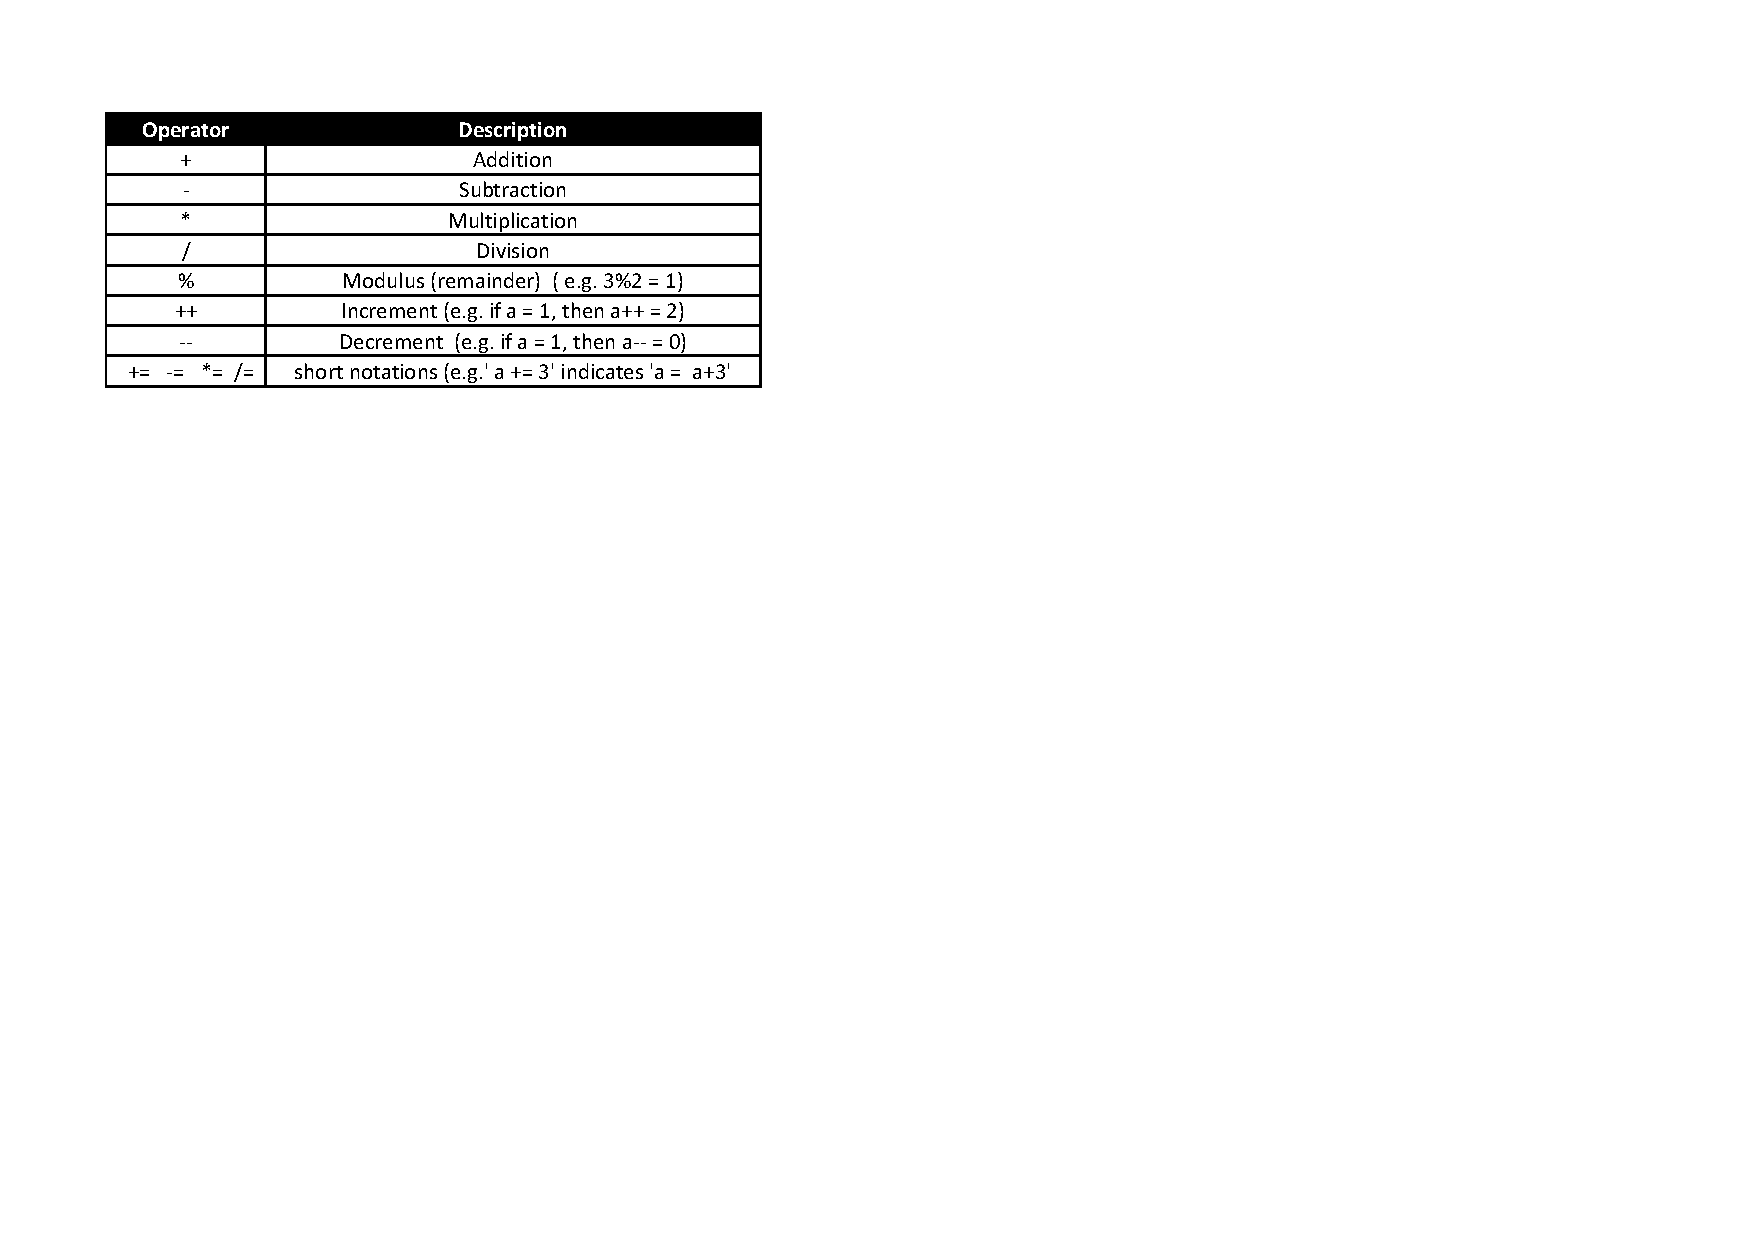
\includegraphics{arithmaticOperator}
	\caption{Arithmetic Operators}
	\label{tbl:arithmaticOperator}
\end{table}

\begin{explanation}[Listing \ref{c:incrementEx}]
	In the listing, the variable `i' is initialized as `1' at Line 7, and printed at Line 9. Next, `i++' operation is printed at Line 12; note that, first `1' is printed by this line; and then the value is increased. This increase in value is verified by print `i' again at Line 13, where the result is 2. Next, `++i' operation is used at Line 16, where the value is increase first and then printed, therefore the result is `3'. Finally, to check the value stored in `i', it is printed again at Line 17.
\end{explanation}
\lstinputlisting[
language = C,
caption    = {Difference in `i++' and `++i'},
label      = {c:incrementEx}
]{incrementEx.c}

\subsection{Relational operators}
Relations operators are used of checking various equality conditions e.g `greater than', `equal' or `less than' etc. These operators are shown in Table \ref{tbl:conditionSymbol}. 

\begin{table}[!h]
	\centering
	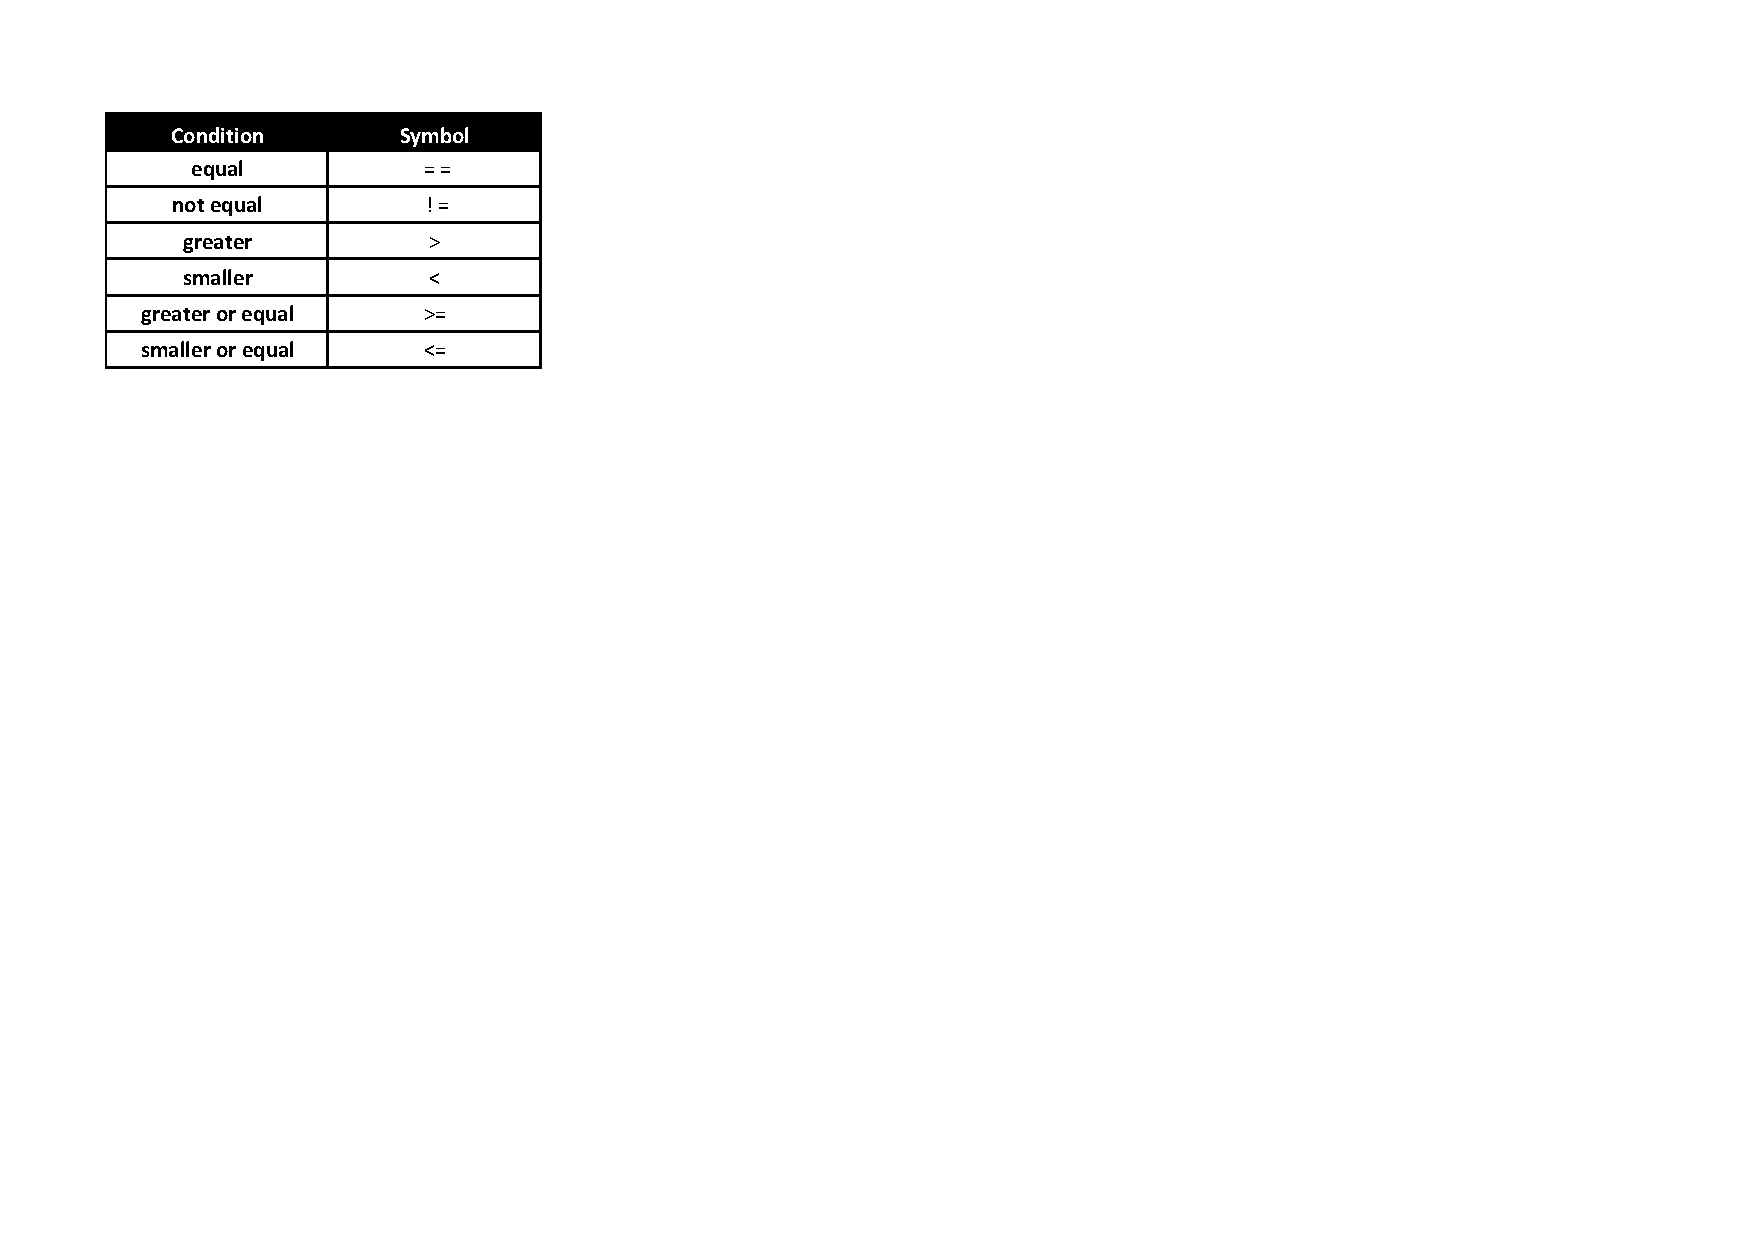
\includegraphics{conditionSymbol}
	\caption{Relational Operators}
	\label{tbl:conditionSymbol}
\end{table}

\subsection{Bitwise operators} 
Bitwise operators are used with boolean data type to calculate the results of boolean expressions or to perform shift operations on boolean data. These operators are shown in Table \ref{tbl:binaryOperators}. Some of these operations are shown in Listing \ref{c:shiftOpEx}. 
\begin{table}[!h]
	\centering
	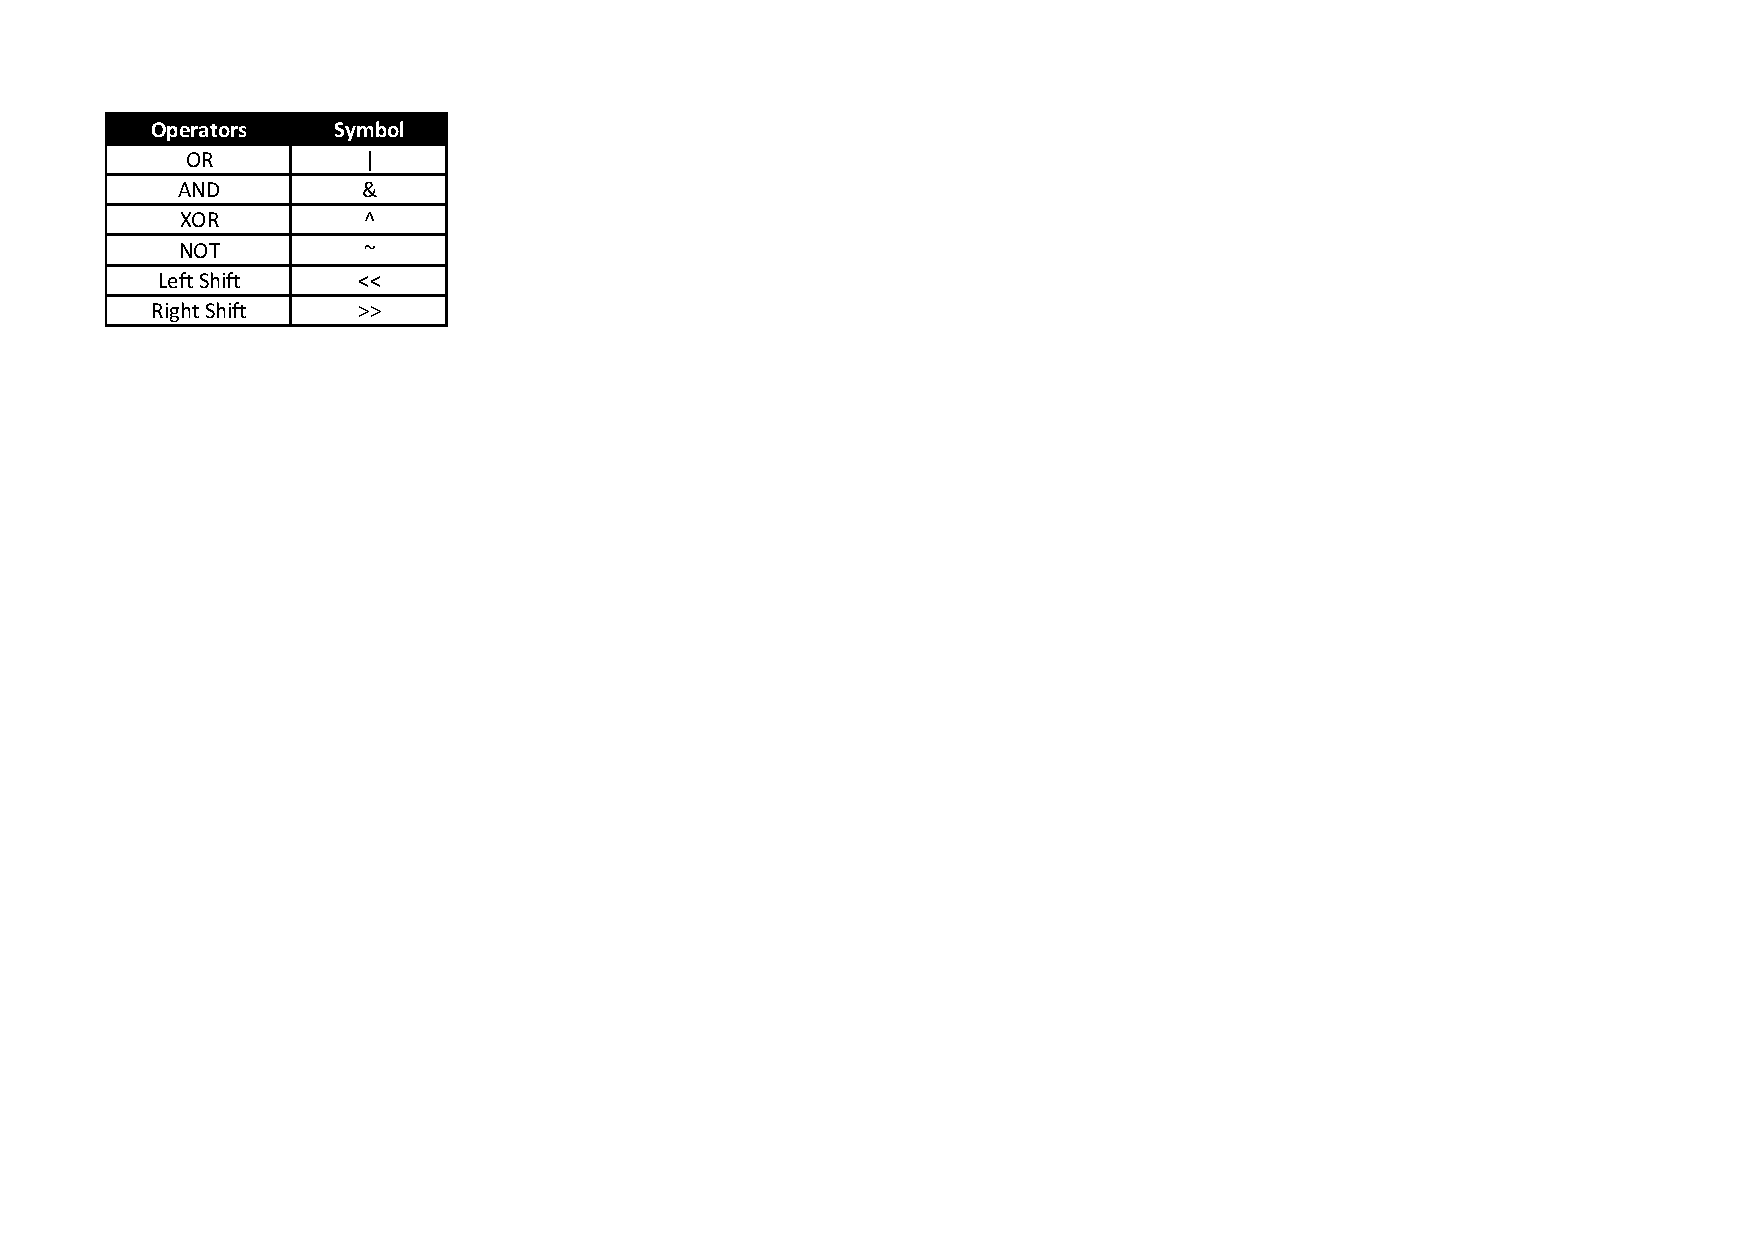
\includegraphics{binaryOperators}
	\caption{Bitwise Operators}
	\label{tbl:binaryOperators}
\end{table}

\begin{explanation}[Listing \ref{c:shiftOpEx}]
	Most of the operations in the listing are straightforward i.e. right shift(Line 12), left shift (Line 13) and xor (Line 17). \textbf{But, look at the `not operation' carefully, it may generate errors in the result in NIOS design}. Since, type `int' is 32 bit long, therefore, a = 2 is saved as `0000-0002' and when `not' operation is performed on it, then result is `ffff-fffd' (not `0000-000d'), at Lines 20-21; therefore, we need to perform `$\&$ (and)' operation with the result, to suppress all the `f' in the result (Line 24). 
\end{explanation}
\lstinputlisting[
language = C,
caption    = {Bitwise operator},
label      = {c:shiftOpEx}
]{shiftOpEx.c}

\subsection{Logical operators}
Logical operators are used to perform logic `and', `or' and `not' operations. Unlike, `bitwise logic operators' these operators do not check the second operator if the first operator gives the result e.g. in `0 \&\& 1 = 0', the result does not depend on the value of second operand i.e. `1'; because first operand is `0', therefore the result will be zero, whether the second operand is `0' or `1'.   
\begin{table}[!h]
	\centering
	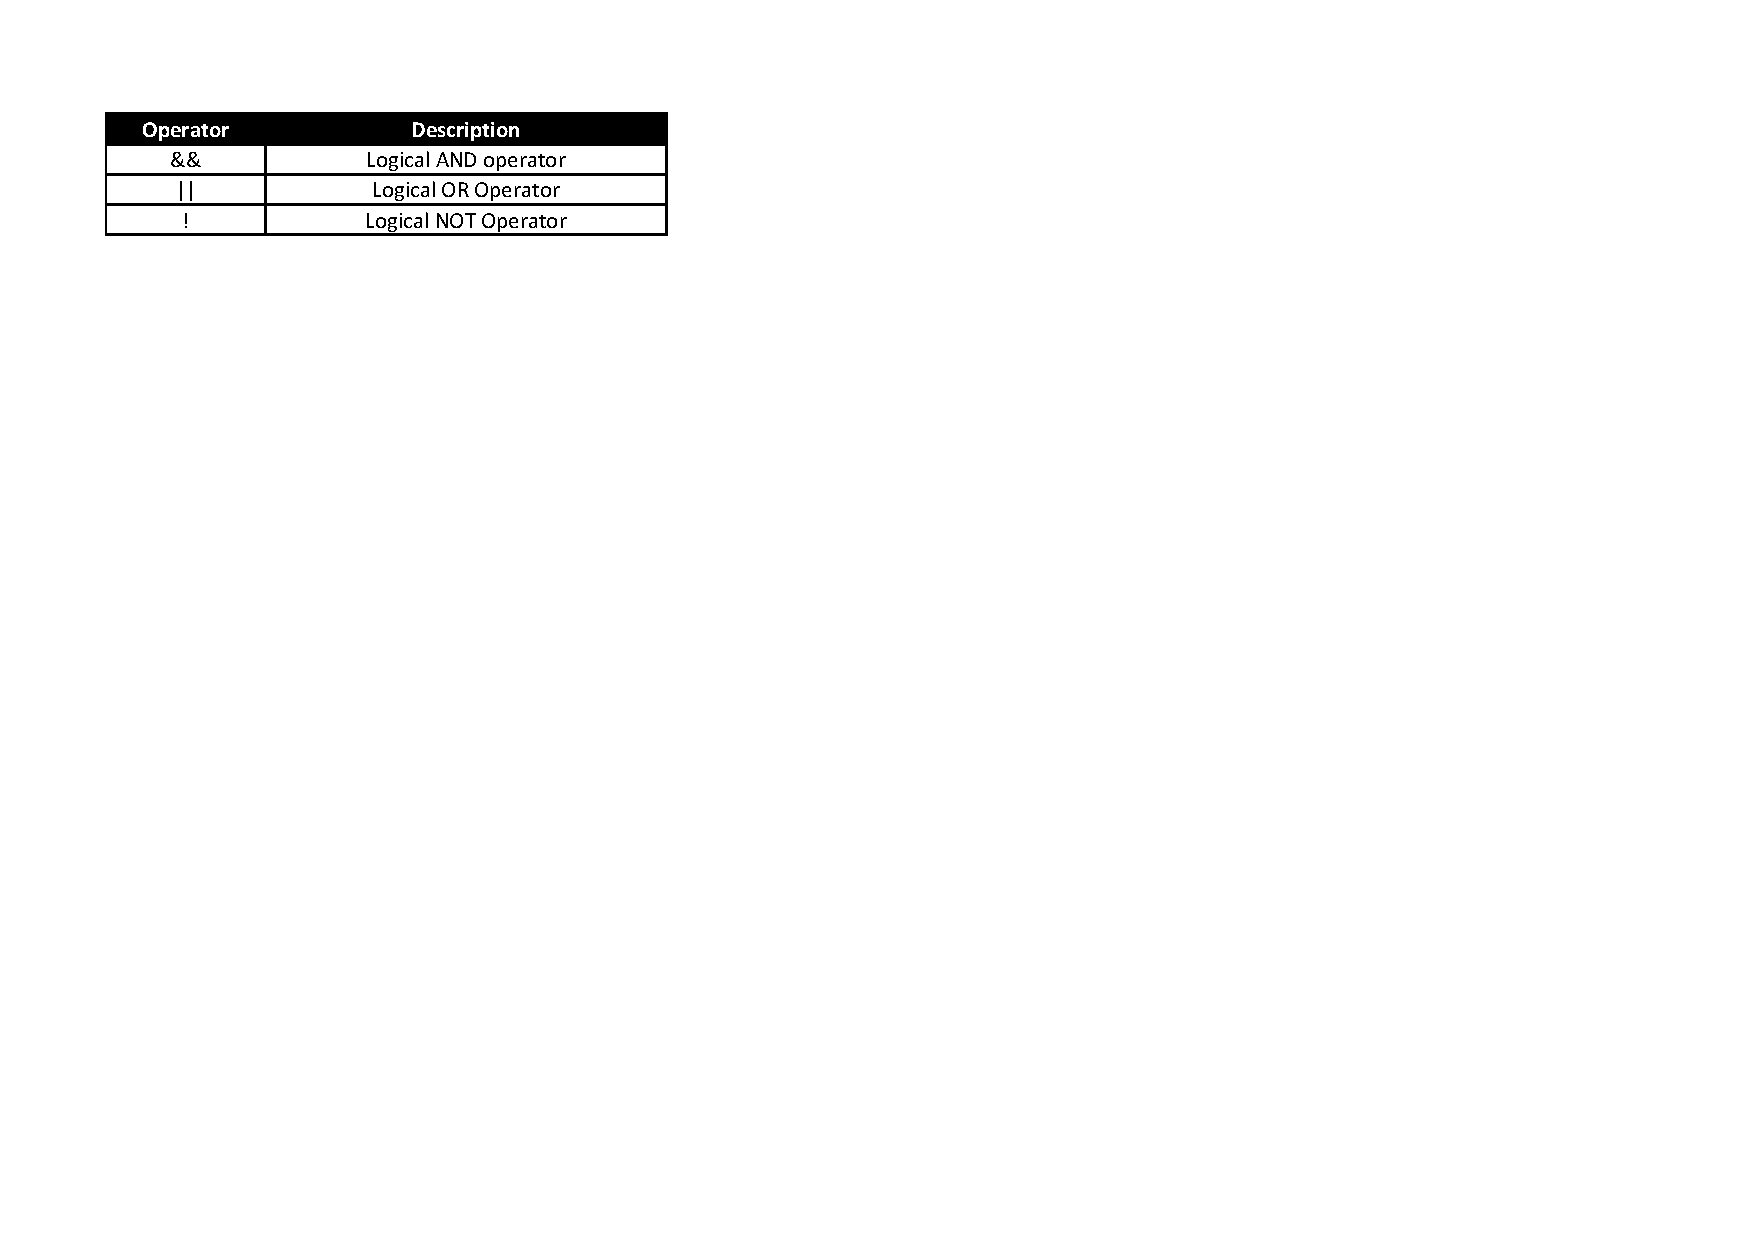
\includegraphics{logicalOperators}
	\caption{Logical Operators}
	\label{tbl:logicalOperators}
\end{table}



\section{Decision statements} \label{decisionStatement}
Control structure can be devided into two categories i.e. decision statements and loops. In this section, simple C codes are presented to explain decision statements available in the language; whereas loops are discussed in next section.

\subsection{If-else statements} \label{sec:ifElse}
\textit{$If-else$} statements are used to define different actions for different conditions. Symbols for such conditions are given in Table \ref{tbl:conditionSymbol}, which can be used as shown in Listing \ref{c:ifEx}. Three examples are shown in this section for three types of statements i.e. \textit{if}, \textit{if-else} and \textit{if- `else if' -else}.


\begin{pyExmp}[If statements]
	Listing \ref{c:ifEx} checks whether the number stored in variable `x' is even or not.
\end{pyExmp}

\begin{explanation}[Listing \ref{c:ifEx}]
	In the listing, variable `x' of type `int' is defined at Line 8; also, this variable is initialize with value 3. In Lines 11 and 17, the `$\%$' sign calculates the remainder of division $x/2$ and checks whether remainder is zero or not respectively. Then, Lines 12-13 will be printed if remainder is zero, else Line 18-19 will be printed. 
	
	Notice that, $\{ \}$ are used with if-statements e.g. at Lines 11 and 14. These brackets tell the compiler that, all the statements within them must be executed only when the condition in corresponding `if' statement is satisfied i.e. 12-13 will be executed, when Line 11 is true. Further, if we remove the brackets from these line, then Line 12 will depend on the `if' statement, whereas Line 13 will be printed all the time. 
\end{explanation}

\lstinputlisting[
language = C,
caption    = {If statement},
label      = {c:ifEx}
]{ifEx.c}


 

\begin{pyExmp}[If-else statement]
	As we know that a number can not be even and odd at the same time. In such cases, we can use if-else statement. Listing \ref{c:ifEx} can be rewritten using `if-else' statement as shown in Listing \ref{c:ifElseEx}.
\end{pyExmp}

\begin{explanation}[Listing \ref{c:ifElseEx}]
	Here, only one condition is specified i.e. at Line 10. Compiler will check this line, if this is true, then Line 11-12 will be printed, otherwise compiler will go to `else' statement at Line 14 and Lines 15-16 will be printed.
\end{explanation}
\lstinputlisting[
language = C,
caption    = {If-else statement},
label      = {c:ifElseEx}
]{ifElseEx.c}

\begin{pyExmp}[`If else-if else']
	In previous case, there were only two conditions which were implemented using `if-else statement'. If there are more than two conditions then `else if' can be used as shown in this example. Further, `if else-if else' block can contain any number of `else-if' statement between one `if' and one `else' statement.  
\end{pyExmp}

\begin{noNumBox}
	Note that, the operator `or' at Line 18 of Listing \ref{c:ElseIfEx}, will generate error, if we execute the code using `gcc ElseIFEx.c -o out', as this operator for C++ compiler only. This code can be executed with command `g++ ElseIFEx.c -o out'. 
\end{noNumBox}

\begin{explanation}[Listing \ref{c:ElseIfEx}]
	In this listing, Line 11 get the value of variable `grade' from the user. The possible value of grades are A, a, B, b,  C, c, D and d. If grade is `A or a', then Line 15 will be printed. Note that, the `or' operation is used in three ways, i.e. `$||$', `$|$' and `or' at Lines 14, 16 and 18 respectively.  If grade value provided by the user is `B or b', then compiler will first check the Line 14, which is false, therefore it will go to next `else-if' statement at Line 16, since it is true, therefore Line 17 will be printed; and compiler will leave the if-block. If we provide the wrong grade, e.g. Z, then compiler will check all the statements i.e. Lines 14, 16, 18 and 20; and finally reach to `else' block and print the Line 23. 
\end{explanation}
\lstinputlisting[
language = C,
caption    = {`If else-if else' statement},
label      = {c:ElseIfEx}
]{ElseIfEx.c}


\begin{pyExmp}[`Nested If else-if else']
	We can use various if statements inside the other if statements, which are known as nested statements. Listing \ref{c:ifElifElse} is the example of nested loop, where divisibility of the number with 2 and 3 is checked.  
\end{pyExmp}
\begin{explanation}[Listing \ref{c:ifElifElse}]
	 The listing checks whether the number is divisible by 2 and 3 using nested if-else statements. Nested statements are used for `if statement' at Line 10. Here, line 10 checks whether the number is division by 2 or not; if divisible, then compiler goes to nested loop (at line 11) and checks whether number is divisible by 3 or not; if divisible, then Line 12 will be printed, else Line 15 and 16 will be printed. Note that, line 16 prints the value of remainder when number is divided by 3. Next, if number is not divisible by 2 (at Line 10), then compiler will directly go to the Line 19; and if number is divisible by 3, then Line 20 will be printed. If number is not divisible by 3 as well, then compiler will go to Line 22 (i.e. else statement) and finally Lines 23-25 will be printed.
\end{explanation}
\lstinputlisting[
language = C,
caption    = {`Nested If else-if else' statement},
label      = {c:ifElifElse}
]{ifElifElse.c}



\subsection{Switch-case-default statements}
Similar to `if statements', the switch-case statements can be used to perform certain operations, only if the specific conditions are met, as shown in Listing \ref{c:switchCase}. 

\begin{explanation}[Listing \ref{c:switchCase}]
	Operation of this listing is same as the Listing \ref{c:ElseIfEx}, but the condition is only checked for uppercase letter. We can add more case-statements for considering the lowercase letters as well. Here, the switch-statement depends on variable `grade' (Line 10); and it is initialized with value `B' at Line 8; and Lines 10-22 are the switch-statement, which contain various `case-statements' (i.e. Lines 11, 14 and 17) and one `default' statement at Line 20. 
	
	When we execute this code, the compiler will reach to `switch statement (Line 10)' and then first go to Line 11 and compare the value of grade i.e. `B' with `A', since these are not equal therefore it will go to next `case statement' at Line 15. Now, the condition is matched, therefore Line 15 will be printed out and then Line 16 will break the execution of switch statement, i.e. the complier will exit from the switch statement and will reach to line 23. `\textbf{Note that, unlike if-else-statements, the compiler does not automatically quit the switch-statement, a separate `break' statement is required to exit the case. If we do not use `break' statement, then compiler will check all the `cases' and finally execute the `default' block. More specifically, we use the `break' statement to avoid the execution of `default' block.}
	
	
\end{explanation}

\lstinputlisting[
language = C,
caption    = {Switch-case statement},
label      = {c:switchCase}
]{switchCase.c}

\subsection{Conditional operator ($? :$)}
	The conditional operator can be used as `if-else' statements as shown Listing \ref{c:conditionalOperatorEx} and \ref{c:conditionalOperatorEx2}. \textbf{In this section, `const char *' is used to define character-array, which is discussed in Section \ref{sec:chArray}}.
	
	\begin{explanation}[Listing \ref{c:conditionalOperatorEx}]
		In conditional operator, the condition is specified before `?' and the `true and false' results are seperated by `:'. For example, in this listing, condition `(a $\%$2)== 0)' is specified before `?' at Line 14. Note that, the result before `:' (i.e. even)  is assigned to variable `result' if the condition is true, otherwise the result after `:' (i.e. odd) will be assigned to variable `result'. Finally, Line 16 will display the message for even or odd number. 
	\end{explanation}
	
	\lstinputlisting[
	language = C,
	caption    = {Condition operator as `if-else' statement},
	label      = {c:conditionalOperatorEx}
	]{conditionalOperatorEx.c}
	
	\begin{explanation}[Listing \ref{c:conditionalOperatorEx2}]
		Conditional operator can be used as `if- else if- else' statement as well. For this, instead of assigning the value for `false condition' after `:', we should put another condition-checking statement; e.g. in the listing, Line 14 ends with `:' and then at Line 15 starts with another condition. Now, if the condition at Line 14 (i.e. a $\%$ == 0) does not satisfy, then condition at Line 15 will be checked. Lastly, if none of the condition is matched, then Line 17 will be printed. 
	\end{explanation}
	\lstinputlisting[
	language = C,
	caption    = {Condition operator as `if-else if-else' statement},
	label      = {c:conditionalOperatorEx2}
	]{conditionalOperatorEx2.c}
	
\section{Loops}
Loops are used to perform the operations repetitively. Three types of loop conditions are discussed in this section i.e. `for loop', `while loop' and `do while loop'. 
\subsection{For loop}

\begin{noNumBox}
	Note that, `int j' inside the `for loop', i.e. Line  13 of Listing \ref{c:forLoop}, will generate error, if we execute the code using `gcc forloop.c -o out', as this operation is only allowed with the C99 or C11 compiler. This code can be executed with command `gcc -std=c99 forLoop.c -o out' or `g++ forloop.c -o out'. 
\end{noNumBox}

\begin{explanation}[Listing \ref{c:forLoop}]
	In the listing, two `for loops' are used i.e. at Line 13 and Line 25. In Line 13, variable `i' is used which is declared at Line 8; and there is only statement inside this loop i.e. Line 14, which prints the value of `i'. First, the loop will start with i = 0 at Line 13 and the statement inside the loop will be printed till the value of i $<$ 5. And after executing the statement at Line 14, the value of the variable `i' will be increased by 1 using `i++' statement in Line 13. When the value of i becomes 5, then compiler will not execute the Line 14 and go outside the loop i.e at Line 16. Then Line 19 prints the current value of `i', whose value is increased to 5, due to `i++' statement in the `for loop' at Line 13.
	
	Loop at Line 25, is similar to Line 13, but `\textbf{int j = 0}' is used here, instead of `\textbf{j = 0}'. This `int' keyword will create a local variable `j' for the loop and will be \textbf{independent} of the variable `j' at Line 8. Hence, the value of `j' printed by the Line 31 will be 2 (not 8). Value is not 8 because the variable `j' which has the value 8 (i.e. `j' at line Line 25) is local to `for loop', and will be discarded by the compiler after coming out of the loop. 

	\textbf{Further, the for loop can be executed in reverse direction as well using `i$--$' operation, as shown in Listing \ref{c:reverseOrder}.}	
\end{explanation}

\begin{noNumBox}
	Note that, for(;;) is used for infinite loop; e.g. if we replace Line 13 with `for(;;)'
	then the loop will continue forever. Use `ctrl+C' to stop the loop.
\end{noNumBox}
	
\lstinputlisting[
language = C,
caption    = {For loop},
label      = {c:forLoop}
]{forLoop.c}

\subsection{While loop}
While loop uses a condition-check statement; and the loop continues till the condition is true, as shown in Listing \ref{c:whileLoop}.

\begin{explanation}[Listing \ref{c:whileLoop}]
	In the listing, the variable `i' is initialized with 0 (Line 8). Then `while loop' is used at Line 10, with condition `(i $<$ 5)', therefore the loop will continue till (i $<$ 5). Further, the loop contains two statements i.e. Line 11 which prints the value of `i' and Line 12 which increments the value of i by 1. When the value of `i' is reached to 5, then the compiler will exit the loop and reach to Line 14. 
	
	\begin{noNumBox}
		Note that, while(1) is used for infinite loop; e.g. if we replace Line 10 with `while(1)'
		then the loop will continue forever. Use `ctrl+C' to stop the loop.
	\end{noNumBox}
\end{explanation}

\lstinputlisting[
language = C,
caption    = {While loop},
label      = {c:whileLoop}
]{whileLoop.c}

\subsection{Do-while loop}
Do-while loop is not very popular method for creating loops, but can be used when we want to execute the statement at least once. 
\begin{explanation}[Listing \ref{c:doWhileLoop}]
	The listing is similar to `while loop', except the condition is stated at the end of the loop i.e. with `while statement' at Line 13. Since, condition is checked at the end of the loop, therefore it guarantees that the loop will execute at least one time. 
\end{explanation}

\lstinputlisting[
language = C,
caption    = {Do-while loop},
label      = {c:doWhileLoop}
]{doWhileLoop.c}

\section{Continue and Break statements}
Continue and Break statements are used with loops, to skip or end the execution of the loop respectively for certain cases. 

\subsection{Continue}
Continue statement is used to skip the loop for certain cases as shown in Listing \ref{c:forContinueLoop}. Here, `continue' statement is used inside the `if statement' (see Lines 12-14); therefore the \textbf{rest of the part} of the loop will be skipped whenever the result of `i$\%$2 is 0' i.e. Line 16 will be skipped. Hence, the values printed are the odd numbers only, as for even number the execution of the loop is skipped. \textbf{In the same way, we can use the `continue statement' with other loops as well.}

\lstinputlisting[
language = C,
caption    = {Continue statement},
label      = {c:forContinueLoop}
]{forContinueLoop.c}

\subsection{Break}
Break statement exit the loop permanently, instead of skipping the loop for certain cases as shown in Listing \ref{c:whileBreakLoop}. Here, break statement is used with `if statement' at Lines 14-16		. Therefore, the compiler will exit from the `while loop' whenever the result of `i$\%$7 is 0'. Hence, the value printed at the output are 0 to 6. \textbf{In the same way, we can use the `continue statement' with other loops as well.}

\lstinputlisting[
language = C,
caption    = {Break statement},
label      = {c:whileBreakLoop}
]{whileBreakLoop.c}

\section{Conclusion}
In this chapter, various examples are shown to understand the operators, conditional statements and loop statements. Also, continue and break statements are discussed which are used to skip and break the loops respectively. 